\section{Máquinas de Turing}
El modelo más básico de una máquina de turing  consiste en un control finito, una cinta infinita dividida en celdas y una cabeza de lectura. Cada celda de la cinta puede contener un único símbolo del alfabeto finito de la cinta.

Inicialmente, la cinta contiene una cadena de símbolos de entrada, seguida de un símbolo especial llamado blanco. La cabeza de lectura se coloca sobre el primer símbolo de la cadena de entrada. La máquina de Turing puede leer y escribir símbolos en la cinta o mover la cabeza de lectura a la izquierda o a la derecha.
\begin{figure}[H]
  \begin{center}
    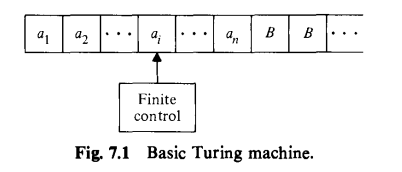
\includegraphics[scale=0.75]{imagenes/mt.png}
  \end{center}
\end{figure}
Formalmente, definimos la máquina de Turing (MT) \(M\) como una tupla:
\[
  M = \langle Q, \Sigma, \Gamma, \delta, q_0, B, F \rangle
\]

Donde:
\begin{itemize}
  \item \(Q\) es un conjunto finito de estados.
  \item \(\Sigma\) es un alfabeto de entrada.
  \item \(\Gamma\) es un alfabeto de cinta.
  \item \(\delta: Q\times\Gamma\to Q\times\Gamma\times\{L, R\}\) es una función de transición. Podría estar indefinido para algunos argumentos. La función indica devuele el estado al que se debe pasar, el símbolo a escribir en la posición actual de la cinta y el movimiento del cabezal (izquierda o derecha).
  \item \(q_0 \in Q\) es el estado inicial.
  \item \(B \in \Gamma\) es el símbolo blanco.
  \item \(F \subseteq Q\) es el conjunto de estados finales.
\end{itemize}

\paragraph{Configuración instantanea:} Una configuración instantánea de una MT es una tupla \(\alpha_1 q \alpha_2\) donde \(q\in Q\) y \(\alpha_1,\alpha_2\in\Gamma^*\) donde:
\begin{itemize}
  \item \(\alpha_1\) son los simbolos de la cinta a la izquierda del cabezal.
  \item \(q\) es el estado actual.
  \item \(\alpha_2\) son los símbolos de la cinta a la derecha del cabezal hasta el último símbolo distinto de \(B\).
\end{itemize}
Notemos que \(\alpha_1,\alpha_2\in\Gamma^*\), osea que pueden tener apariciones de \(B\).

Asumismos que el cabezal está escaneando el símbolo más a la derecha de \(\alpha_2\) o un blanco si \(\alpha_2=\lambda\).

\paragraph{Movimiento del cabezal:} El movimiento del cabezal se define como sigue: Sea \[X_1\dots X_{i-2}qX_{i}\dots X_n\]una configuración instantánea de una MT \(M\).

Supongamos que \(\delta(q,X_i) = (p, Y, L)\):
\begin{itemize}
  \item Si \(i -1 = n\), asumimos \(X_i = B\)
  \item Si \(i = 1\) entonces es imposible moverse a la izquierda.
  \item Si \(1 < i < n\) entonces escribimos:
        \[
          X_1\dots X_{i-1}qX_{i}\dots X_n \underset{M}{\vdash} X_1\dots X_{i-2}pX_{i-1}YX_{i+1}\dots X_n
        \]

        En caso de haya algún sufijo de \(X_{i-1}YX_{i+1}\dots X_n\) que sea completamente blanco, entonces se elimina.
\end{itemize}

Similarmente, si \(\delta(q,X_i) = (p, Y, R)\):
\[
  X_1\dots X_{i-1}qX_{i}\dots X_n \underset{M}{\vdash} X_1\dots X_{i-1}YpX_{i+1}\dots X_n
\]

Si dos configuraciónes instantáneas están relacionadas por \(\resulta{M}\), entonces decimos que la segunda es un resultado de la primera.

Si una configuración instantánea resulta de otra en un número fínito de pasos, entonces están relacionadas por el símbolo \(\resultam{M}\).

\paragraph{Lenguaje aceptado por una MT:} Definimos al lenguaje aceptado por una MT \(M=\langle Q, \Sigma, \Gamma, \delta, q_0, B, F \rangle\) como:
\[
  \mathcal{L}(M) = \{ \omega \in \Sigma^*  : q_0\omega \resultam{M} \alpha_1 p\alpha_2 \text{ con } p\in F \land \alpha_1,\alpha_2\in\Gamma^* \}
\]

Asumimos que la máquina de Turing se detiene cuando el input es aceptado. Además es posible que nunca se detenga si el input no es aceptado.

\subsection{Autómatas linealmente acotados}
Es una máquina de Turing  no deterministica que cumple con las siguientes condiciones:
\begin{enumerate}
  \item El alfabeto de entrada incluye dos símbolos especiales (\textcentoldstyle~y \textdollar) que son utilizados como topes izquierdo y derecho, respectivamente.
  \item El autómata no se mueve ni a la izquierda de \textcentoldstyle ni a la derecha de \textdollar, ni los sobreescribe.
\end{enumerate}

\subsubsection{Máquinas de dos cintas}
Una máquina de Turing con dos o más cintas puede simularse usando la defición dada anteriormente. Para ello, definimos los estados en \(\Gamma\) como tuplas \([x_1, x_2]\) donde \(x_i\) sería el símbolo guardado en la \(i\)-ésima cinta.


\begin{teorema}
  Si \(L\) es un lenguaje dependiente del contexto, entonces existe un autómata linealmente acotado \(A\) tal que \(\mathcal{L}(A) = L\).
\end{teorema}

\begin{demo}[0.8\textwidth]
  Se construye el autómata linealmente acotado \(M\) tal que:
  \begin{enumerate}
    \item La primera cinta contiene la cadena de entrada \textcentoldstyle\(\omega\)\textdollar.
    \item La segunda cinta se utiliza para generar las formas de la derivación. En cualquie instante, esta cinta contendrá la forma sentencial \(\alpha\) que representa la derivación de la cadena de entrada. Se inicializa con el símbolo distingido \(S\).
  \end{enumerate}

  El autómata funcionará de la siguientes manera:
  \begin{enumerate}
    \item Si \(\omega=\lambda\), entonces \(M\) se detiene rechanzando la cadena de entrada.
    \item Sino:
          \begin{enumerate}
            \item Selecciona (en forma no deterministica) la posición \(i\) dentro de \(\alpha\) (la derivación que se encuentra en la cinta)
            \item Selecciona (en forma no deterministica) la producción \(\beta\to\gamma\in P\).
            \item Si \(\beta\) aparece a partir de la posición \(i\) en \(\alpha\), entonces remplaza \(\beta\) por \(\gamma\) en \(\alpha\).
            \item Si la nueva forma sentencial \(\alpha\) es tal que \(|\alpha| > |\omega|\), entonces \(M\) se detiene rechazando la cadena de entrada.
            \item Sino, comparamos \(\alpha\) con \(\omega\). Si son iguales, entonces \(M\) se detiene aceptando la cadena de entrada. Sino, se vuelve a repetir el paso 2.
          \end{enumerate}
  \end{enumerate}
\end{demo}

\subsubsection{Lenguajes recursivos}
Son lenguajes \(L\) sobre un alfabeto \(\Sigma\) para el cual existe una máquina de Turing que se detiene para todo \(\alpha\in\Sigma^*\) y la acepta (termina en un estado final) si \(\alpha\in L\) o la rechaza (termina en un estado no final) si \(\alpha\notin L\). En otras palabras, son los lenguajes para los cuales existe un algoritmo que permite decidir la pertenencia (o no) de toda cadena al lenguaje.

\begin{teorema}\label{teorema:recursividad}
  Todo lenguaje dependiente del contexto es recursivo
\end{teorema}

\begin{demo}[0.8\textwidth]
  Sea \(G=\langle N, \Sigma, P, S \rangle\) un gramática dependiente del contexto y \(\omega\in\Sigma^*\). Vamos a construir un grafo fínito en el cual cada nodo tiene asocida un \(\alpha\in(V_N\cup V_T)^+\) con \(|\alpha| \leq |\omega|\). Las arista representas una producción de \(G\), osea si \(\gamma_1\tau\gamma_2\) y \(\gamma_1\beta\gamma_2\) son dos nodos, entonces van a estar conectados si y solo si \(\tau\to\beta\in P\).

  Por ser \(G\) dependiente del contexto, vale \(|\tau|\leq |\beta|\), entonces \(|\gamma_1\tau\gamma_2|\leq |\gamma_1\beta\gamma_2|\). Por lo tanto, el grafo es acotado.

  En este grafo finito, es cierto que \(S\underset{G}{\deriva}\omega\) si y solo si existe un camino desde el nodo correspondiente a \(S\) hasta el nodo correspondiente a \(\omega\). Y esto último es decidible, o sea, tiene algoritmo. Por lo tanto, \(G\) es recursivo.
\end{demo}

\begin{lemma}
  Sea \(M_1, M_2, \dots\) una enumeración de un conjunto de máquinas de Turing que paran para todas las entadradas. Siempre existe un lenguaje recursivo que no es aceptado por ninguna de ellas, o sea, siempre existe un lenguaje \(L\) tal que \(L\) es recursivo y \(L\notin\mathcal{L}(M_i)\) para todo \(i\).
\end{lemma}

\begin{demo}[0.8\textwidth]
  Consideremos el lenguaje definido \( L = \{ \omega_i : \omega_i \notin \mathcal{L}(M_i)\}\), es decir \(L\) está formado por todas las cadenas que son rechazadas por alguna de las máquinas \(M_i\). Como es decidible si \(\omega_i\in L\) o no (pues simplemente corremos las \(M_i\) con entrada \(\omega\) y vemos si para en un estado no final), entonces \(L\) es recursivo.

  Supongamos ahora que este lenguaje es aceptado por alguna de las máquinas enumeradas. Sea \(M_j\), la misma. Entonces ¿que pasa si \(\omega_j\in L\)?

  Por definición de \(L\) tenemos que \(w_j\in L \iff w_j\notin \mathcal{L}(M_j) \iff w_j \notin L\). Esto es un absurdo, por lo tanto \(L\) no es aceptado por ninguna máquina \(M_1,M_2,\dots\).
\end{demo}

\begin{lemma}
  Existe un lenguaje recursivo que no es dependiente del contexto
\end{lemma}
\begin{demo}[0.8\textwidth]
  Vamos a tratar de demostrar que podemos encontrar una numeración de máquinas Turing correspondientes a cada uno de los lenguajes dependientes del contexto definidos sobre \(\{0,1\}^*\).
\end{demo}
\begin{demoPart}[0.8\textwidth]
  Estas máquinas de Turing paran en todas las entradas porque como los lenguajes son dependientes de contexto, siempre hay un algoritmo de reconomcimiento cuando el lenguaje es dependiente del contexto.

  Codifiquemos todas estas gramaticas con cadenas binarias, es decir, demos una representación binaria a cada símbolo de la gramática codificando:

  \begin{itemize}
    \item \(0 = 10\)
    \item \(1 = 100\)
    \item y al resto de los simbolos \(s_k = 10^k\)
  \end{itemize}

  Gracias a esta codificación mediante 0s y 1s, podemos enumerarlas de la siguientes manera: \(G_1,G_2,\dots\). Además, por el teorema \ref{teorema:recursividad}, existen autómatas \(M_1, M_2,\dots\) que aceptan los lenguajes generados por cada una de ellas.

  Luego, por el lema, anterior, tenemos que existe un lenguaje \(L\) recursivo que no es aceptado por ninguno de estos autómatas y no es dependiente del contexto.
\end{demoPart}

\begin{teorema}
  Sea \(M\) una máquina de Turing no deterministica y \(L = \mathcal{L}(M)\). Entonces existe una máquina de Turing determinista \(M'\) que acepta el mismo lenguaje.
\end{teorema}

\begin{demo}[0.8\textwidth]
  Sea \(r\) la máxima cantidad posible de transiciones que parte de un estado cualquiera de \(M\).

  Para cada estado, numeremos las transiciones que parten de él con números entre \(1\) y \(r\) como máximo. Entonces toda secuencia finita de enteros entre \(1\) y \(r\) puede ser interpretada como una secuencia de transiciones en la \(M\), partiendo desde el estado inicial (algunas de estas secuencias no serán ejecutables ya que puede llegar a no existir alguna de las transiciones).

  Entonces podemos contruir una máquina de Turing \(M'\) de tres cintas tal que:
  \begin{itemize}
    \item La primer cinta contiene la cadena de entrada, la cual no será modificada.
    \item La segunda contendrá una secuencia de enteros entre \(1\) y \(r\) que corresponderá a una secuencia de transiciones a partir del estado inicial.
    \item La terecera servirá para simular la máquina no-deterministica \(M\).
  \end{itemize}

  La máquina \(M'\) funcionará de la siguiente manera:
  \begin{enumerate}
    \item Para cada secuencia de enteros entre \(1\) y \(r\):
          \begin{itemize}
            \item Escribe la secuencia en la cinta 2.
            \item Borra el contenido de la cinta 3.
            \item Simula \(M\) con la secuencia de transiciones escrita en la cinta 2.
            \item Si se acepta la cadena de la cinta \(1\) en esa simulación, entonces el \(M'\) termina en estado de aceptación. Sinó volvemos a repetir con otra secuencia
          \end{itemize}
          Cuando la cadena analizada no es aceptada por \(M\) entonces, \(M'\) no se detendrá nunca.
  \end{enumerate}
\end{demo}

\subsection{Gramáticas sin restricciones}
\begin{teorema}
  Sea \(G=\langle V_N, V_T, P, S \rangle\) una gramática sin restricciones, tal que \(L = \mathcal{L}(M)\), entonces existe una máquina de Turing \(M\) tal que \(L = \mathcal{L}(M)\).
\end{teorema}
\begin{demo}[0.8\textwidth]
  Vamos a construir una máquina de Turing no determinista de dos cintas tal que:
  \begin{itemize}
    \item La primera contiene la cadena de entrada \(w\).
    \item La segunda contiene la forma sentencial \(\alpha\) de la derivación de la cadena de entrada. Se inicializa con el símbolo inicial distinguido \(S\).
  \end{itemize}
\end{demo}
\begin{demoPart}[0.8\textwidth]
  La máquina de Turing funcionará de la siguiente manera:
  \begin{itemize}
    \item Seleccionar (en forma no-deterministica) la posición \(i\) dentro de \(\alpha\) (en la cinta 2)
    \item Seleccionar (en forma no-deterministica) la regla de producción \(\beta \rightarrow \gamma\in P\) que se puede aplicar en la posición \(i\).
    \item Si \(\beta\) aparece a partir de la posición \(i\) en \(\alpha\), entonces se reemplaza por \(\gamma\) en \(\alpha\).
    \item Se compara la nueva forma sentencial \(\alpha\) con la candea de entrada \(w\). Si coinciden, entonces se acepta la cadena. Sino se vuelve a repetir el proceso
  \end{itemize}
\end{demoPart}

\begin{teorema}
  Si una máquina de Turing \(M\) acepta un lenguaje \(L\), entonces existe una gramática sin restricciones \(G\) tal que \(L = \mathcal{L}(G)\).
\end{teorema}
\begin{demo}[0.8\textwidth]
  La idea es que \(G\) gnere dos copias de alguna representación de la cadena de entrada y que luego simule la opreación de \(M\) sobre una de ellas. Si esta simulación resulta en una aceptación, entonces la primera copia se en convierte en la cadena igual a la de la entrada.

  Si \(M=(Q, \Sigma, \delta, q_0, B, F)\) entonces \(G = \langle V_N, \Sigma, P, A_1 \rangle\) con:
  \begin{enumerate}
    \item \(V_N = ((\Sigma\cup\{\lambda\})\times\Gamma)\cup\{A_1,A_2,A_3\}\)
    \item \(P\) contiene las producciones:
          \begin{enumerate}
            \item \(A_1 \to q_0A_2\)
            \item \(A_2 \to [a,a]A_2\) para cada \(a\in\Sigma\)
            \item \(A_2\to A_3\)
            \item \(A_3\to [\lambda, B]A_3\)
            \item \(A_3\to\lambda\)
            \item \(q[\alpha,X]\to[\alpha, Y]p\) para todo \(a\in\Sigma\cup\{\lambda\}\), \(q\in Q\) y \(X,Y\in\Gamma\) tal que \(\delta(q,X) = (p, Y, R)\)
            \item \([b,Z]q[a,X]\to p[b,Z][a,Y]\) para todo \(a,b\in\Sigma\cup\{\lambda\}\), \(q\in Q\) y \(X, Y, Z\in\Gamma\) tals que \(\delta(q, X) = (p, Y, L)\)
            \item \([a,X]q\to qaq\), \(q[a,X]\to qaq\), \(q\to\lambda\) para todo \(a\in\Sigma\cup\{\lambda\}\), \(q\in F\) y \(X\in\Gamma\).
          \end{enumerate}

          Utilizando las reglas \(1\) y \(2\) se puede generar \(A_1 \deriva q_0[a_1, a_1]\dots[a_n, a_n]A_2\).
  \end{enumerate}
\end{demo}
\begin{demoPart}[0.8\textwidth]
  Luego utilizando la regla 3 se generan los símbolos correspondientes a los espacios en blanco necesarios para el análisis de la cadena de entrada en \(M\): \[A_1\deriva q_0[a_1,a_1]\dots[a_n,a_n][\lambda, B]^mA3\]
  Utilizando las reglas 6 y 7 se simula la opreación de \(M\) sobre las segundas componentes, dejando intactas las primeras componentes. Puede \red{demostrarse} que
  \begin{align*}
     & q_0a_1\dots a_n\resultam{M} X_1\dots X_{r-1}qX_r\dots X_s \\ &\implies q_0[a_1,a_1]\dots[a_n,a_n][\lambda, B]^m \deriva [a_1, X_1]\dots[a_{r-1},X_{r-1}]q[a_r, X_r]
  \end{align*}

  con \(a_1,\dots,a_n\in\Sigma\) y \(a_{n+1} = \dots = a_{n+m} = \lambda \), \(X_1,\dots, X_{n+m}\in\Gamma\) y \(X_{s+1} =\dots = X_{n+m} = B\). Lo que deseamos probar es cierto cunado la cantidad de transiciones en \(M\) es cero, porque en este caso tenemos \(r =1\) y \(s = n\).

  Tomemos ahora el caso de \(k\) transacciones:

  \[ q_0a_1\dots a_n\overset{k-1}{\resulta{M}} X_1\dots X_{r-1}qX_r\dots X_s \resulta{M} Y_1\dots Y_{t-1}pY_r\dots Y_u \]

  por hipotesís inductiva tenemos que:

  \begin{align*}
     & q_0[a_1,a_1]\dots[a_n,a_n][\lambda, B]^m                                   \\
     & \deriva [a_1, a_1]\dots[a_{r-1},X_{r-1}]q[a_r, X_r]\dots[a_{n+m}, X_{n+m}]
  \end{align*}

  Si en el paso \(k\) el movimiento es hacia la derecha, entonces \(\delta(q,X_r) = (p, Y, R)\), tenemos que \(t=r+1\) y por la regla \(6\) sabemos \(q[a_r,X_r]\to[a_r, Y_r]p \in P\) por lo que:

  \begin{align*}
     & [a_1, a_1]\dots[a_{r-1},X_{r-1}]q[a_r, X_r]\dots[a_{n+m}, X_{n+m}]          \\
     & \deriva [a_1, a_1]\dots[a_r, Y_r]p[a_{r+1}, X_{r+1}]\dots[a_{n+m}, X_{n+m}]
  \end{align*}

  Si en el paso \(k\) el movimiento es hacia la izquierda, entonces \(\delta(q,X_r) = (p, Y, L)\), tenemos que \(t=r-1\) y por la regla \(7\) sabemos \([a_{r-1},X_{r-1}]q[a_r,X_r]\to p[a_{r-1},X_{r-1}][a_r,Y_r] \in P\) por lo que:
  \begin{align*}
     & [a_1, a_1]\dots[a_{r-1},X_{r-1}]q[a_r, X_r]\dots[a_{n+m}, X_{n+m}]                          \\
     & \deriva [a_1, a_1]\dots[a_{r-2}, X_{r-2}]p[a_{r-1},X_{r-1}][a_r,Y_r]\dots[a_{n+m}, X_{n+m}]
  \end{align*}

  Entonces, si llegamos a una forma sentencian en la que el estado \(q\) sea final, aplicando repetidas veces la regla 8 tenquemos que queda
\end{demoPart}

\begin{demoPart}[0.8\textwidth]
  \[
    [a_1, Y_1]\dots[a_{t-1},Y_{t-1}]q[a_t, Y_t]\dots[a_{n+m}, Y_{n+m}] \deriva a_1\dots a_{n}.
  \]
  En el sentido inverso, \red[puede demostrarse] también que, para toda cadena \(\alpha\in\mathcal(L)(G)\) vale que \(x\in\mathcal{L}(M)\).
\end{demoPart}

\subsection{Lenguajes recursivos enumerables
Son los lenguajes para los cuales se puede decir si una cadena pertenece al mismo pero no se puede asegurar que una cadena no pertenezca al mismo.

Las máquinas de Turing para estos lenguajes van a parar y aceptar una cadena si está pertenece al lenguaje. Pero si pasamos una cadena que no pertenece podrían entrar en un loop infinito en vez de parar y rechazar.

\begin{teorema}
  Existe un lenguaje que no es recursivamente enumerable
\end{teorema}

\paragraph{Lenguaje universal:} \(L_u\) es el lenguaje \(\langle M, \omega\rangle\) donde \(M\) es una máquina de Turing y \(\omega\in\mathcal{L}(M)\), osea:

\[
  L_u = \{ \langle M, \omega\rangle \mid M \text{ es una máquina de Turing y } \omega \in \mathcal{L}(M) \}
\]

\begin{teorema}
  El lenguaje universal \(L_u\) es recursivamente enumerable.
\end{teorema}

\begin{demo}
  \red{demostrar?}
\end{demo}